\documentclass[../Interim_Report_Master]{subfiles}
\begin{document}
\hypertarget{op_imp}{\section{OpenCL Implementation}\label{op_imp}}
The initial testing of numerical methods and the model were performed in Python as this language allows for prototype code to be quickly produced due to its simplicity and feature rich libraries such as NumPy. Python also features capability for creating GPU code through the PyOpenCL library \cite{pyopencl}. However, the existing code uses C and OpenCL to build executable files for running simulations. 

\subsection{Additions made to the Code}
The implementation of the heat and mass model was through adding the required code to the cut down code that was tested in Section \ref{v_and_v}.

\subsubsection{Source Code Structure}
For the sake of clarity the existing source code structure is shown in Figure \ref{demorange_struct} which can be found in Section \ref{prog_strut}. The new source code structure with DEM functionality removed and the heat and mass model included is shown in Figure \ref{hmorange_struct}. 
\begin{figure}[H]
	\centering
	\includegraphics*[width=0.5\textwidth, trim=0 985 0 0, clip]{./Diagrams/HMOranges_Structure/HMOranges_Structure.pdf}
\end{figure}
\begin{figure}
	\centering
	\includegraphics*[width=0.5\textwidth, trim=0 290 0 330, clip]{./Diagrams/HMOranges_Structure/HMOranges_Structure.pdf}
\end{figure}
\begin{figure}
	\centering
	\includegraphics*[width=0.5\textwidth, trim=0 0 0 1025, clip]{./Diagrams/HMOranges_Structure/HMOranges_Structure.pdf}
	\caption{File structure of the HMOranges source code.}
	\label{hmorange_struct}
\end{figure}

\subsubsection{Variables}
As already mentioned the DEM code had to be stripped out. Once this was completed and results from the code verified and validated the heat and mass transfer methods could be added. This involved adding the following set of new variables to the particle structure:
\begin{multicols}{3}
\begin{itemize}
	\item T\_d
	\item W\_V
	\item T\_B
	\item L\_V
	\item C\_L
	\item P\_atm
	\item R\_bar
	\item R
	\item W\_G
	\item theta\_1
	\item theta\_2
	\item Y\_G
	\item Pr\_G
	\item Sc\_G
	\item f\_2
	\item P\_G
	\item T\_G
	\item H\_deltaT
	\item m\_d
	\item Reynolds\_d
	\item initial\_mass
	\item rho\_G
\end{itemize} 
\end{multicols}

In addition to this code was added to the \lstinline[style=cstyleintext]|createNormalDistVelocities| function that initialises the particles so the extra required variables are set to the required initial conditions. Finally, the equations to solve the heat and mass transfer were added to the iterate particle kernel. This included adding a stop condition for updating the particle properties. Namely: position, speed, temperature and mass. When the current particle mass reaches $1\%$ of its starting mass, all properties for the particle are set to zero. At each further timestep the value of the particle properties is logged as zero. This makes later data analysis easier as particles are identified by a row of data in the text file. So the number of rows has to remain the same. This is especially important for utilising Paraview which identifies particles by row.  

\subsubsection{Heat and Mass Transfer Model}
The heat and mass transfer model as outlined in Section \ref{drop_mod} was implemented slightly differently to Python. The OpenCL code uses a single kernel to iterate the particles and this contains the functionality to evaluate the model.

\subsection{Verification and Validation}
Similar to the Python code the OpenCl code must undergo verification and validation tests to ensure the equations are being solved correctly.

For the verification tests in Sections \ref{sec:uc_mass_opencl} and \ref{sec:uc_temp_opencl} the settings used are as per Table \ref{tab:sim_set_uc}.

\subsubsection{Uncoupled Heat Transfer}
Figure \ref{plot:uc_heat_v_opencl} shows the uncoupled heat transfer for a range of timesteps with the numerical solution converging to the analytic solution with decreasing timestep. As an implicit method has been used the numerical solution under predicts the analytic solution and this can also be clearly seen.

\begin{figure}[H]
	\centering
	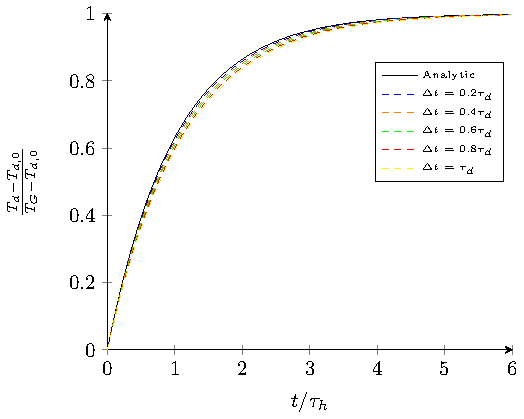
\includegraphics[width=0.8\textwidth]{./Diagrams/Uncoupled_Heat_Transfer_Verification/Uncoupled_Heat_Transfer.pdf}
	\caption{$T_d$ for a droplet sized $D^2=1.1mm$ with $Re_d=0$, $T_{d_0}=282K$, $T_G=298K$.}
	\label{plot:uc_heat_v_opencl}
\end{figure}

\subsubsection{Uncoupled Mass Transfer}\label{sec:uc_mass_opencl}
For the mass transfer non-dimensionalised droplet diameter squared has been plotted in Figure \ref{plot:uc_mass_v_opencl}. Like the uncoupled heat transfer plot it can be seen the numerical solution converges to the analytic solution for decreasing timestep size.
\begin{figure}[H]
	\centering
	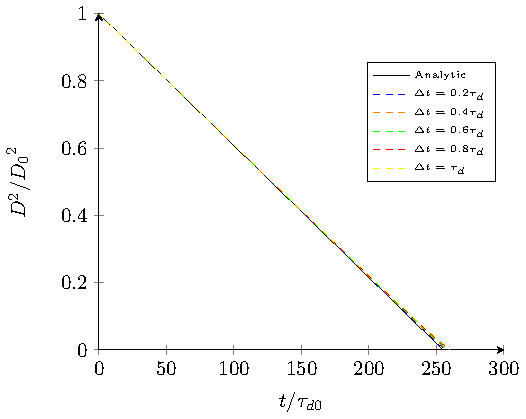
\includegraphics[width=0.8\textwidth]{./Diagrams/Uncoupled_Mass_Transfer_Verification/Uncoupled_Mass_Transfer.pdf}
	\caption{$T_d$ for a droplet sized $D^2=1.1mm$ with $Re_d=0$, $T_{d_0}=282K$, $T_G=298K$.}
	\label{plot:uc_mass_v_opencl}
\end{figure}


\subsubsection{Coupled Heat and Mass Transfer}\label{sec:uc_temp_opencl}
The coupled heat and mass results are plotted in Figure \ref{coupled_d2_water} and Figure \ref{coupled_heat_water}. The settings used can be found in Tables \ref{tab:sim_set_uc}, \ref{tab:sim_set_hex} and \ref{tab:sim_set_dec}. As with Section \ref{sec:heat_mass_val} these show good agreement with the results in the literature. 
\begin{figure}[H]
	\centering
	\begin{subfigure}{\textwidth}
		\centering
		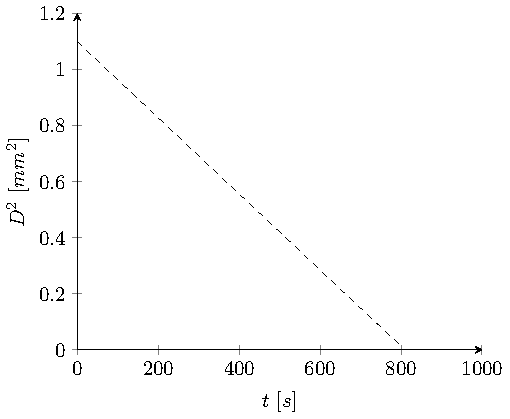
\includegraphics[width=0.8\textwidth]{./Diagrams/Coupled_Heat_Mass_Transfer_Verification/Coupled_D2_Transfer_Water.pdf}
		\caption{}
		\label{coupled_d2_water}
	\end{subfigure}
\end{figure}
\begin{figure}\ContinuedFloat
	\centering
	\begin{subfigure}{\textwidth}
		\centering
		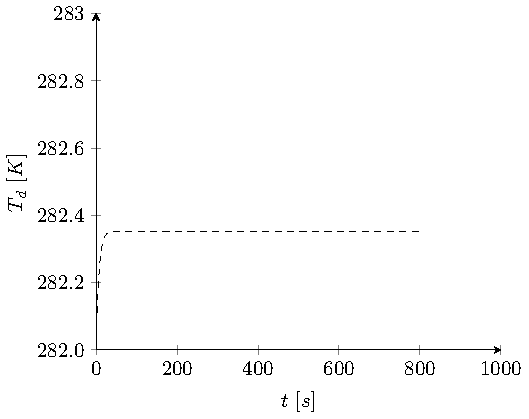
\includegraphics[width=0.8\textwidth]{./Diagrams/Coupled_Heat_Mass_Transfer_Verification/Coupled_Heat_Transfer_Water.pdf}
		\caption{}
		\label{coupled_heat_water}
	\end{subfigure}
	\caption{Droplet diameter squared (a) and droplet temperature (b) temporal evolution for a water droplet sized $D^2=1.1mm$ with $Re_d=0$, $T_{d_0}=282K$, $T_G=298K$, $Y_G=0$ and $\Delta t=\tau_{d0}/64$.}
\end{figure}

As with Section \ref{sec:heat_mass_val} additional results for hexane and decane were produced. These results are included in the Section \ref{cl_extra_res} of the Appendix. The results presented there are in agreement with those from the Python code. 
\end{document}